\documentclass[]{book}
\usepackage{lmodern}
\usepackage{amssymb,amsmath}
\usepackage{ifxetex,ifluatex}
\usepackage{fixltx2e} % provides \textsubscript
\ifnum 0\ifxetex 1\fi\ifluatex 1\fi=0 % if pdftex
  \usepackage[T1]{fontenc}
  \usepackage[utf8]{inputenc}
\else % if luatex or xelatex
  \ifxetex
    \usepackage{mathspec}
  \else
    \usepackage{fontspec}
  \fi
  \defaultfontfeatures{Ligatures=TeX,Scale=MatchLowercase}
\fi
% use upquote if available, for straight quotes in verbatim environments
\IfFileExists{upquote.sty}{\usepackage{upquote}}{}
% use microtype if available
\IfFileExists{microtype.sty}{%
\usepackage{microtype}
\UseMicrotypeSet[protrusion]{basicmath} % disable protrusion for tt fonts
}{}
\usepackage[margin=1in]{geometry}
\usepackage{hyperref}
\hypersetup{unicode=true,
            pdftitle={Paystack},
            pdfauthor={Edgar John},
            pdfborder={0 0 0},
            breaklinks=true}
\urlstyle{same}  % don't use monospace font for urls
\usepackage{natbib}
\bibliographystyle{apalike}
\usepackage{color}
\usepackage{fancyvrb}
\newcommand{\VerbBar}{|}
\newcommand{\VERB}{\Verb[commandchars=\\\{\}]}
\DefineVerbatimEnvironment{Highlighting}{Verbatim}{commandchars=\\\{\}}
% Add ',fontsize=\small' for more characters per line
\usepackage{framed}
\definecolor{shadecolor}{RGB}{248,248,248}
\newenvironment{Shaded}{\begin{snugshade}}{\end{snugshade}}
\newcommand{\KeywordTok}[1]{\textcolor[rgb]{0.13,0.29,0.53}{\textbf{#1}}}
\newcommand{\DataTypeTok}[1]{\textcolor[rgb]{0.13,0.29,0.53}{#1}}
\newcommand{\DecValTok}[1]{\textcolor[rgb]{0.00,0.00,0.81}{#1}}
\newcommand{\BaseNTok}[1]{\textcolor[rgb]{0.00,0.00,0.81}{#1}}
\newcommand{\FloatTok}[1]{\textcolor[rgb]{0.00,0.00,0.81}{#1}}
\newcommand{\ConstantTok}[1]{\textcolor[rgb]{0.00,0.00,0.00}{#1}}
\newcommand{\CharTok}[1]{\textcolor[rgb]{0.31,0.60,0.02}{#1}}
\newcommand{\SpecialCharTok}[1]{\textcolor[rgb]{0.00,0.00,0.00}{#1}}
\newcommand{\StringTok}[1]{\textcolor[rgb]{0.31,0.60,0.02}{#1}}
\newcommand{\VerbatimStringTok}[1]{\textcolor[rgb]{0.31,0.60,0.02}{#1}}
\newcommand{\SpecialStringTok}[1]{\textcolor[rgb]{0.31,0.60,0.02}{#1}}
\newcommand{\ImportTok}[1]{#1}
\newcommand{\CommentTok}[1]{\textcolor[rgb]{0.56,0.35,0.01}{\textit{#1}}}
\newcommand{\DocumentationTok}[1]{\textcolor[rgb]{0.56,0.35,0.01}{\textbf{\textit{#1}}}}
\newcommand{\AnnotationTok}[1]{\textcolor[rgb]{0.56,0.35,0.01}{\textbf{\textit{#1}}}}
\newcommand{\CommentVarTok}[1]{\textcolor[rgb]{0.56,0.35,0.01}{\textbf{\textit{#1}}}}
\newcommand{\OtherTok}[1]{\textcolor[rgb]{0.56,0.35,0.01}{#1}}
\newcommand{\FunctionTok}[1]{\textcolor[rgb]{0.00,0.00,0.00}{#1}}
\newcommand{\VariableTok}[1]{\textcolor[rgb]{0.00,0.00,0.00}{#1}}
\newcommand{\ControlFlowTok}[1]{\textcolor[rgb]{0.13,0.29,0.53}{\textbf{#1}}}
\newcommand{\OperatorTok}[1]{\textcolor[rgb]{0.81,0.36,0.00}{\textbf{#1}}}
\newcommand{\BuiltInTok}[1]{#1}
\newcommand{\ExtensionTok}[1]{#1}
\newcommand{\PreprocessorTok}[1]{\textcolor[rgb]{0.56,0.35,0.01}{\textit{#1}}}
\newcommand{\AttributeTok}[1]{\textcolor[rgb]{0.77,0.63,0.00}{#1}}
\newcommand{\RegionMarkerTok}[1]{#1}
\newcommand{\InformationTok}[1]{\textcolor[rgb]{0.56,0.35,0.01}{\textbf{\textit{#1}}}}
\newcommand{\WarningTok}[1]{\textcolor[rgb]{0.56,0.35,0.01}{\textbf{\textit{#1}}}}
\newcommand{\AlertTok}[1]{\textcolor[rgb]{0.94,0.16,0.16}{#1}}
\newcommand{\ErrorTok}[1]{\textcolor[rgb]{0.64,0.00,0.00}{\textbf{#1}}}
\newcommand{\NormalTok}[1]{#1}
\usepackage{longtable,booktabs}
\usepackage{graphicx,grffile}
\makeatletter
\def\maxwidth{\ifdim\Gin@nat@width>\linewidth\linewidth\else\Gin@nat@width\fi}
\def\maxheight{\ifdim\Gin@nat@height>\textheight\textheight\else\Gin@nat@height\fi}
\makeatother
% Scale images if necessary, so that they will not overflow the page
% margins by default, and it is still possible to overwrite the defaults
% using explicit options in \includegraphics[width, height, ...]{}
\setkeys{Gin}{width=\maxwidth,height=\maxheight,keepaspectratio}
\IfFileExists{parskip.sty}{%
\usepackage{parskip}
}{% else
\setlength{\parindent}{0pt}
\setlength{\parskip}{6pt plus 2pt minus 1pt}
}
\setlength{\emergencystretch}{3em}  % prevent overfull lines
\providecommand{\tightlist}{%
  \setlength{\itemsep}{0pt}\setlength{\parskip}{0pt}}
\setcounter{secnumdepth}{5}
% Redefines (sub)paragraphs to behave more like sections
\ifx\paragraph\undefined\else
\let\oldparagraph\paragraph
\renewcommand{\paragraph}[1]{\oldparagraph{#1}\mbox{}}
\fi
\ifx\subparagraph\undefined\else
\let\oldsubparagraph\subparagraph
\renewcommand{\subparagraph}[1]{\oldsubparagraph{#1}\mbox{}}
\fi

%%% Use protect on footnotes to avoid problems with footnotes in titles
\let\rmarkdownfootnote\footnote%
\def\footnote{\protect\rmarkdownfootnote}

%%% Change title format to be more compact
\usepackage{titling}

% Create subtitle command for use in maketitle
\newcommand{\subtitle}[1]{
  \posttitle{
    \begin{center}\large#1\end{center}
    }
}

\setlength{\droptitle}{-2em}

  \title{Paystack}
    \pretitle{\vspace{\droptitle}\centering\huge}
  \posttitle{\par}
    \author{Edgar John}
    \preauthor{\centering\large\emph}
  \postauthor{\par}
      \predate{\centering\large\emph}
  \postdate{\par}
    \date{2019-02-24}

\usepackage{booktabs}

\begin{document}
\maketitle

{
\setcounter{tocdepth}{1}
\tableofcontents
}
\chapter{Brief Introduction}\label{brief-introduction}

This book is the official documentation for the
\href{https://paystack.com/}{Paystack} R Package

The Package can be found at \url{https://github.com/ebinabo/paystack}

It contains

\begin{itemize}
\tightlist
\item
  wrappers for the official
  \href{https://developers.paystack.co/v1.0/reference\#paystack-inline-x}{Paystack
  API}
\item
  a few helper functions and a lot more coming soon \ldots{}
\end{itemize}

To use this you would need to open a
\href{https://dashboard.paystack.com/\#/signup}{Paystack account} and
have developer option set to true while signing up.

You would need your own API Keys to use this package and they can be
found \href{https://dashboard.paystack.com/\#/settings/developer}{here}

This book is still under development, functions would be added over time
as updates are made. A very quick intro could be found
\href{https://bookdown.org/edgarjohn95/paystack/how-to-rpubs.html\#/}{here}

If you have any issues using this package, you could submit your issue
\href{https://github.com/ebinabo/paystack/issues/new}{here}

\chapter{Installation}\label{installation}

I'll put this up on CRAN sometime toon so it's easier to install but
before then, you could get it any of the ways listed below

\section{From GitHub}\label{from-github}

To install this package run

\begin{Shaded}
\begin{Highlighting}[]
\NormalTok{devtools}\OperatorTok{::}\KeywordTok{install_github}\NormalTok{(}\StringTok{"ebinabo/paystack"}\NormalTok{)}
\end{Highlighting}
\end{Shaded}

\section{Manual Installation}\label{manual-installation}

I understand newer versions of RStudio don't handle downloading from
github properly so I've included a
\href{https://github.com/ebinabo/paystack/blob/master/manual_installation.R}{manual\_installation}
script as well.

Instructions on installing it are included there

Please unzip the file to your downloads or anywhere but the reserved
folder in \textasciitilde{}Documents/R/win-lib/version folder, took me
some time to figure that out

\chapter{Basics}\label{basics}

\section{General Function Structure}\label{general-function-structure}

The API wrappers have the same general function structure

\begin{Shaded}
\begin{Highlighting}[]
\KeywordTok{_function_name}\NormalTok{(authoriaztion, path_param, ...)}
\end{Highlighting}
\end{Shaded}

\begin{itemize}
\tightlist
\item
  \textbf{authorization} : Header tag containing your secret or public
  keys
\item
  \textbf{path\_param} : A slug that's added to the url to return a
  specific response
\item
  \textbf{\ldots{}} : Body parameters that also return a specific
  response
\end{itemize}

You could see a list of them at the Available Objects chapter

\section{Getting Help}\label{getting-help}

The functions are properly documented and you can view them from within
RStudio by running \texttt{?\_function\_name}

An example of this would be

\begin{Shaded}
\begin{Highlighting}[]
\NormalTok{?request_reauthorization}
\end{Highlighting}
\end{Shaded}

which would display

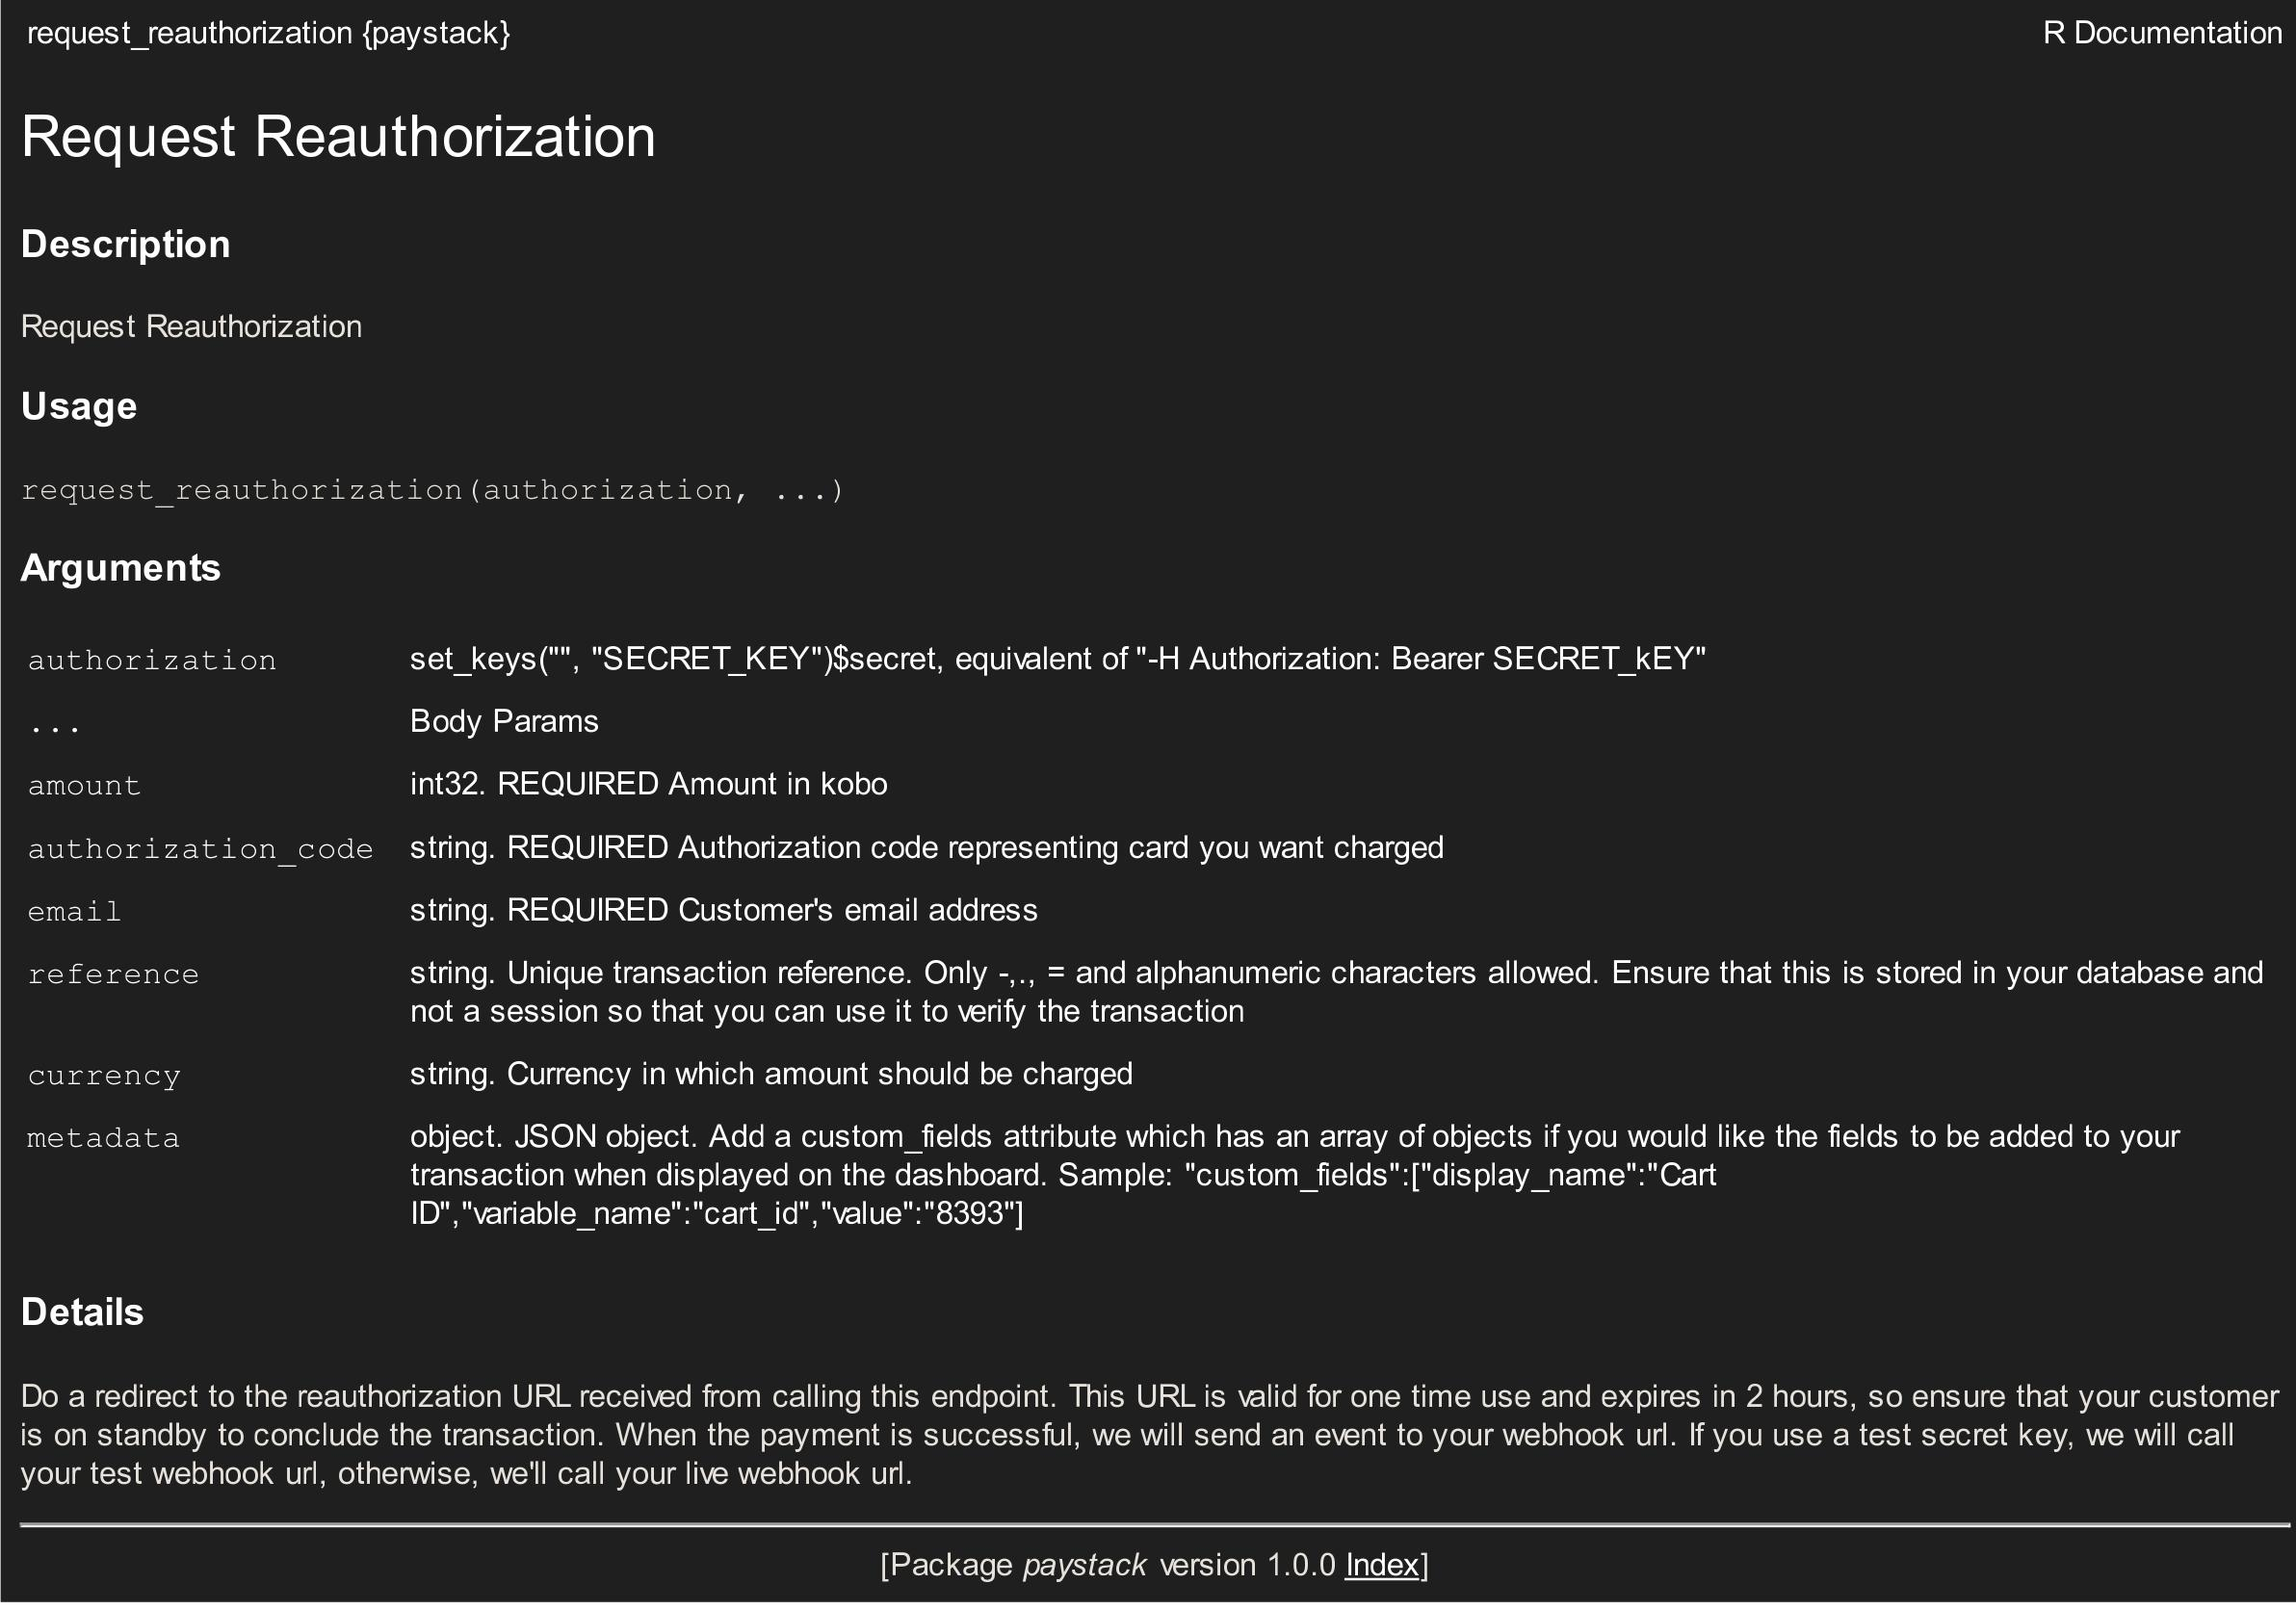
\includegraphics[width=33.11in]{img/help-page}

The body params could be found at this
\href{https://developers.paystack.co/v1.0/reference\#paystack-inline-x}{reference
page}.

ps: I'm still updating the documentation for the help pages in the
package so you might need to check the main reference page linked above
for the mean time.

\chapter{Set Keys}\label{set-keys}

From the API reference page, we would notice that the curl commands
contain header tags

\begin{itemize}
\tightlist
\item
  -H ``Authorization: Bearer SECRET\_KEY''
\item
  -H ``Content-Type: application/json''
\end{itemize}

This package uses http verbs from the
\href{https://httr.r-lib.org}{httr} package and by default,
``Content-Type: application/json'' is added to the headers of all the
functions already.

The following sections decribe how you could use this function

\begin{Shaded}
\begin{Highlighting}[]
\CommentTok{# load required libraries}
\KeywordTok{library}\NormalTok{(paystack)}
\KeywordTok{library}\NormalTok{(magrittr)}
\end{Highlighting}
\end{Shaded}

\section{Basic Usage}\label{basic-usage}

Running \texttt{set\_keys(public\_key,\ secret\_key)} returns a list of
two \texttt{\textless{}request\textgreater{}} objects

\begin{Shaded}
\begin{Highlighting}[]
\NormalTok{auth <-}\StringTok{ }\KeywordTok{set_keys}\NormalTok{(}\StringTok{"pk_mode_publ1ck3y"}\NormalTok{, }\StringTok{"sk_mode_s3cr3tk3y"}\NormalTok{)}
\NormalTok{auth}
\end{Highlighting}
\end{Shaded}

\begin{verbatim}
## $secret
## <request>
## Headers:
## * Authorization: Bearer sk_mode_s3cr3tk3y
## 
## $public
## <request>
## Headers:
## * Authorization: Bearer pk_mode_publ1ck3y
\end{verbatim}

To use with any function in the package which takes in an arg
authorization, run

\begin{Shaded}
\begin{Highlighting}[]
\KeywordTok{_function_name}\NormalTok{(}\DataTypeTok{authorization =}\NormalTok{ auth}\OperatorTok{$}\NormalTok{secret, other_args)}
\end{Highlighting}
\end{Shaded}

\section{Using RDS files}\label{using-rds-files}

RDS stands for R Data Structure, these files let you store R objects in
a file to access them or share them.

It is not recomended you share these files with anyone outside your
company because they hold your authorization details from paystack.

However, putting them in your project directory would make it easier for
you to reuse the keys.

In a case where you would want to put your project on a public repo on
github, you might want to leave out this file as well as your .RData
workspace image and your .Rhistory files which might contain traces of
your keys.

These files have a file ext of .rda, don't forget to include.

To save the object,

\begin{Shaded}
\begin{Highlighting}[]
\KeywordTok{set_keys}\NormalTok{(}\StringTok{"pk_mode_publ1ck3y"}\NormalTok{, }\StringTok{"sk_mode_s3cr3tk3y"}\NormalTok{) }\OperatorTok\StringTok{ }
\StringTok{  }\KeywordTok{saveRDS}\NormalTok{(}\StringTok{"path_to_file.rda"}\NormalTok{)}
\end{Highlighting}
\end{Shaded}

To read it,

\begin{Shaded}
\begin{Highlighting}[]
\KeywordTok{readRDS}\NormalTok{(}\StringTok{"path_to_file.rda"}\NormalTok{)}
\end{Highlighting}
\end{Shaded}

\chapter{Available Objects}\label{available-objects}

\section{Functions}\label{functions}

\begin{Shaded}
\begin{Highlighting}[]
\CommentTok{# get all the function names from paystack package}
\NormalTok{function_names <-}\StringTok{ }\KeywordTok{unclass}\NormalTok{(}\KeywordTok{lsf.str}\NormalTok{(}\DataTypeTok{envir =} \KeywordTok{asNamespace}\NormalTok{(}\StringTok{"paystack"}\NormalTok{), }\DataTypeTok{all =}\NormalTok{ T))}
\CommentTok{# for every element in function_names, get the args the function accepts}
\NormalTok{function_args <-}\StringTok{ }\KeywordTok{map}\NormalTok{(function_names, formalArgs)}
\CommentTok{# set names of function_args accordingly}
\KeywordTok{names}\NormalTok{(function_args) <-}\StringTok{ }\NormalTok{function_names}

\NormalTok{function_args}
\end{Highlighting}
\end{Shaded}

\begin{verbatim}
## $archive_invoice
## [1] "authorization" "invoice_id"   
## 
## $charge_authorization
## [1] "authorization" "..."          
## 
## $check_authorization
## [1] "authorization" "..."          
## 
## $check_balance
## [1] "authorization"
## 
## $check_pending_charge
## [1] "authorization" "reference"    
## 
## $check_slug_availability
## [1] "authorization" "slug"         
## 
## $create_customer
## [1] "authorization" "..."          
## 
## $create_invoice
## [1] "authorization" "..."          
## 
## $create_page
## [1] "authorization" "..."          
## 
## $create_plan
## [1] "authorization" "..."          
## 
## $create_refund
## [1] "authorization" "..."          
## 
## $create_subaccount
## [1] "authorization" "..."          
## 
## $create_subscription
## [1] "authorization" "..."          
## 
## $create_transfer_recipient
## [1] "authorization" "..."          
## 
## $deactivate_authorization
## [1] "authorization" "..."          
## 
## $delete_transfer_recipients
## [1] "authorization" "recipient_id" 
## 
## $disable_otp
## [1] "authorization"
## 
## $disable_subscription
## [1] "authorization" "..."          
## 
## $enable_otp
## [1] "authorization"
## 
## $enable_subscription
## [1] "authorization" "..."          
## 
## $exchange_rate
## [1] "amount"         "base_currency"  "quote_currency"
## 
## $export_transactions
## [1] "authorization" "..."          
## 
## $fetch_bulk_charge_batch
## [1] "authorization" "batch_id"     
## 
## $fetch_charges_in_batch
## [1] "authorization" "batch_id"      "..."          
## 
## $fetch_customer
## [1] "authorization" "customer_code" "..."          
## 
## $fetch_page
## [1] "authorization" "page_id"      
## 
## $fetch_payment_session_timeout
## [1] "authorization"
## 
## $fetch_plan
## [1] "authorization" "plan_id"      
## 
## $fetch_refund
## [1] "authorization" "trans_id"     
## 
## $fetch_settlements
## [1] "authorization" "..."          
## 
## $fetch_subaccount
## [1] "authorization" "subacct_id"   
## 
## $fetch_subscription
## [1] "authorization" "id"           
## 
## $fetch_transaction
## [1] "authorization" "id"           
## 
## $fetch_transfer
## [1] "authorization" "..."          
## 
## $finalize_disable_otp
## [1] "authorization" "..."          
## 
## $finalize_invoices
## [1] "authorization" "invoice_id"    "..."          
## 
## $get_invoice_metrics
## [1] "authorization"
## 
## $initialize_transaction
## [1] "authorization" "..."          
## 
## $initiate_bulk_charge
## [1] "authorization" "reference"     "..."          
## 
## $initiate_bulk_transfer
## [1] "authorization" "..."          
## 
## $initiate_transfer
## [1] "authorization" "..."          
## 
## $list_banks
## [1] "authorization" "..."          
## 
## $list_bulk_charge_batches
## [1] "authorization" "..."          
## 
## $list_customers
## [1] "authorization" "..."          
## 
## $list_invoices
## [1] "authorization" "..."          
## 
## $list_pages
## [1] "authorization" "..."          
## 
## $list_plans
## [1] "authorization" "..."          
## 
## $list_refunds
## [1] "authorization" "..."          
## 
## $list_subaccount
## [1] "authorization" "..."          
## 
## $list_subscriptions
## [1] "authorization" "..."          
## 
## $list_transactions
## [1] "authorization" "..."          
## 
## $list_transfer_recipients
## [1] "authorization" "..."          
## 
## $mark_as_paid
## [1] "authorization" "invoice_id"    "..."          
## 
## $parse_response
## [1] "response"
## 
## $pause_bulk_charge_batch
## [1] "authorization" "batch_code"   
## 
## $request_reauthorization
## [1] "authorization" "..."          
## 
## $resend_otp
## [1] "authorization" "..."          
## 
## $resolve_account_number
## [1] "authorization" "..."          
## 
## $resolve_bvn
## [1] "authorization" "bvn"          
## 
## $resolve_card_bin
## [1] "card_bin"
## 
## $resolve_phone_number
## [1] "authorization" "..."          
## 
## $resume_bulk_charge_batch
## [1] "authorization" "batch_code"   
## 
## $send_notification
## [1] "authorization" "invoice_id"    "..."          
## 
## $set_keys
## [1] "public_key" "secret_key"
## 
## $set_risk_action
## [1] "authorization" "..."          
## 
## $submit_birthday
## [1] "authorization" "..."          
## 
## $submit_otp
## [1] "authorization" "..."          
## 
## $submit_phone
## [1] "authorization" "..."          
## 
## $submit_pin
## [1] "authorization" "..."          
## 
## $transaction_totals
## [1] "authorization" "..."          
## 
## $update_customer
## [1] "authorization" "id"            "..."          
## 
## $update_invoice
## [1] "authorization" "invoice_id"    "..."          
## 
## $update_page
## [1] "authorization" "page_id"       "..."          
## 
## $update_payment_session_timeout
## [1] "authorization"
## 
## $update_plan
## [1] "authorization" "plan_id"       "..."          
## 
## $update_subaccount
## [1] "authorization" "subacct_id"    "..."          
## 
## $update_transfer_recipients
## [1] "authorization" "recipient_id"  "..."          
## 
## $verify_invoice
## [1] "authorization" "invoice_id"   
## 
## $verify_transaction
## [1] "authorization" "reference"    
## 
## $view_invoice
## [1] "authorization" "invoice_id"   
## 
## $view_transaction_timeline
## [1] "authorization" "id"
\end{verbatim}

\section{Other Objects}\label{other-objects}

\begin{Shaded}
\begin{Highlighting}[]
\CommentTok{# remove function_names from all available objects in the package}
\KeywordTok{setdiff}\NormalTok{(}\KeywordTok{ls}\NormalTok{(}\StringTok{"package:paystack"}\NormalTok{), function_names)}
\end{Highlighting}
\end{Shaded}

\begin{verbatim}
## [1] "available_urls" "banks"          "pay_with_banks" "test_cards"    
## [5] "urls"
\end{verbatim}

\subsection{available\_urls}\label{available_urls}

\begin{Shaded}
\begin{Highlighting}[]
\NormalTok{available_urls}
\end{Highlighting}
\end{Shaded}

\begin{verbatim}
##  [1] "https://api.paystack.co/bank"                               
##  [2] "https://api.paystack.co/bank/resolve"                       
##  [3] "https://api.paystack.co/bank/resolve_bvn"                   
##  [4] "https://api.paystack.co/bulkcharge"                         
##  [5] "https://api.paystack.co/bulkcharge/pause"                   
##  [6] "https://api.paystack.co/bulkcharge/resume"                  
##  [7] "https://api.paystack.co/charge"                             
##  [8] "https://api.paystack.co/charge/submit_birthday"             
##  [9] "https://api.paystack.co/charge/submit_otp"                  
## [10] "https://api.paystack.co/charge/submit_phone"                
## [11] "https://api.paystack.co/charge/submit_pin"                  
## [12] "https://api.paystack.co/customer"                           
## [13] "https://api.paystack.co/customer/deactivate_authorization"  
## [14] "https://api.paystack.co/customer/set_risk_action"           
## [15] "https://api.paystack.co/decision/bin"                       
## [16] "https://api.paystack.co/page"                               
## [17] "https://api.paystack.co/page/check_slug_availability"       
## [18] "https://api.paystack.co/paymentrequest"                     
## [19] "https://api.paystack.co/paymentrequest/archive"             
## [20] "https://api.paystack.co/paymentrequest/finalize"            
## [21] "https://api.paystack.co/paymentrequest/notify"              
## [22] "https://api.paystack.co/paymentrequest/totals"              
## [23] "https://api.paystack.co/paymentrequest/verify"              
## [24] "https://api.paystack.co/plan"                               
## [25] "https://api.paystack.co/refund"                             
## [26] "https://api.paystack.co/settlement"                         
## [27] "https://api.paystack.co/subaccount"                         
## [28] "https://api.paystack.co/subscription"                       
## [29] "https://api.paystack.co/subscription/disable"               
## [30] "https://api.paystack.co/subscription/enable"                
## [31] "https://api.paystack.co/transaction"                        
## [32] "https://api.paystack.co/transaction/charge_authorization"   
## [33] "https://api.paystack.co/transaction/check_authorization"    
## [34] "https://api.paystack.co/transaction/export"                 
## [35] "https://api.paystack.co/transaction/initialize"             
## [36] "https://api.paystack.co/transaction/request_reauthorization"
## [37] "https://api.paystack.co/transaction/timeline"               
## [38] "https://api.paystack.co/transaction/totals"                 
## [39] "https://api.paystack.co/transaction/verify"                 
## [40] "https://api.paystack.co/transfer"                           
## [41] "https://api.paystack.co/transfer/disable_otp"               
## [42] "https://api.paystack.co/transfer/disable_otp_finalize"      
## [43] "https://api.paystack.co/transfer/enable_otp"                
## [44] "https://api.paystack.co/transfer/finalize_transfer"         
## [45] "https://api.paystack.co/transfer/resend_otp"                
## [46] "https://api.paystack.co/transferreceipient"                 
## [47] "https://api.paystack.co/verifications"
\end{verbatim}

\subsection{banks}\label{banks}

\begin{Shaded}
\begin{Highlighting}[]
\NormalTok{banks}
\end{Highlighting}
\end{Shaded}

\begin{verbatim}
##                        name                     slug code payable
## 1               Access Bank              access-bank  044    TRUE
## 2              ALAT by WEMA             alat-by-wema 035A    TRUE
## 3     ASO Savings and Loans               asosavings  401   FALSE
## 4          Citibank Nigeria         citibank-nigeria  023   FALSE
## 5              Diamond Bank             diamond-bank  063   FALSE
## 6           Ecobank Nigeria          ecobank-nigeria  050   FALSE
## 7  Ekondo Microfinance Bank ekondo-microfinance-bank  562   FALSE
## 8           Enterprise Bank          enterprise-bank  084   FALSE
## 9             Fidelity Bank            fidelity-bank  070    TRUE
## 10    First Bank of Nigeria    first-bank-of-nigeria  011   FALSE
## 11 First City Monument Bank first-city-monument-bank  214    TRUE
## 12      Guaranty Trust Bank      guaranty-trust-bank  058    TRUE
## 13            Heritage Bank            heritage-bank  030   FALSE
## 14                Jaiz Bank                jaiz-bank  301   FALSE
## 15            Keystone Bank            keystone-bank  082   FALSE
## 16          MainStreet Bank          mainstreet-bank  014   FALSE
## 17            Parallex Bank            parallex-bank  526   FALSE
## 18             Polaris Bank             polaris-bank  076   FALSE
## 19            Providus Bank            providus-bank  101   FALSE
## 20        Stanbic IBTC Bank        stanbic-ibtc-bank  221   FALSE
## 21  Standard Chartered Bank  standard-chartered-bank  068   FALSE
## 22            Sterling Bank            sterling-bank  232    TRUE
## 23            Suntrust Bank            suntrust-bank  100   FALSE
## 24    Union Bank of Nigeria    union-bank-of-nigeria  032    TRUE
## 25   United Bank For Africa   united-bank-for-africa  033   FALSE
## 26               Unity Bank               unity-bank  215    TRUE
## 27                Wema Bank                wema-bank  035   FALSE
## 28              Zenith Bank              zenith-bank  057    TRUE
\end{verbatim}

\subsection{pay\_with\_banks}\label{pay_with_banks}

\begin{Shaded}
\begin{Highlighting}[]
\NormalTok{pay_with_banks}
\end{Highlighting}
\end{Shaded}

\begin{verbatim}
##                       name code
## 1              Access Bank  044
## 2             ALAT by WEMA 035A
## 3            Fidelity Bank  070
## 4 First City Monument Bank  214
## 5      Guaranty Trust Bank  058
## 6            Sterling Bank  232
## 7    Union Bank of Nigeria  032
## 8               Unity Bank  215
## 9              Zenith Bank  057
\end{verbatim}

\subsection{test\_cards}\label{test_cards}

\begin{Shaded}
\begin{Highlighting}[]
\NormalTok{test_cards}
\end{Highlighting}
\end{Shaded}

\begin{verbatim}
## $no_validation
## $no_validation$card_number
## [1] 4.084084e+15
## 
## $no_validation$exp_date
## [1] "03/21"
## 
## $no_validation$cvv
## [1] 408
## 
## 
## $pin_only_validation
## $pin_only_validation$card_number
## [1] 5.078508e+17
## 
## $pin_only_validation$exp_date
## [1] "03/21"
## 
## $pin_only_validation$cvv
## [1] 81
## 
## $pin_only_validation$pin
## [1] 1111
## 
## 
## $simulated_error_msg
## $simulated_error_msg$error_001
## $simulated_error_msg$error_001$error_message
## [1] "Declined"
## 
## $simulated_error_msg$error_001$card_number
## [1] 4.08408e+15
## 
## $simulated_error_msg$error_001$exp_date
## [1] "03/21"
## 
## $simulated_error_msg$error_001$CVV
## [1] 1
## 
## 
## $simulated_error_msg$error_002
## $simulated_error_msg$error_002$error_message
## [1] "Token Not Generated. Customer Not Registered on Token Platform"
## 
## $simulated_error_msg$error_002$card_number
## [1] 5.078508e+17
## 
## $simulated_error_msg$error_002$exp_date
## [1] "03/21"
## 
## $simulated_error_msg$error_002$cvv
## [1] 82
## 
## $simulated_error_msg$error_002$pin
## [1] 6503
## 
## 
## 
## $simulated_issues
## $simulated_issues$issue_003
## $simulated_issues$issue_003$issue
## [1] "Timeout error"
## 
## $simulated_issues$issue_003$card_number
## [1] 5.06066e+15
## 
## $simulated_issues$issue_003$exp_date
## [1] "03/21"
## 
## $simulated_issues$issue_003$CVV
## [1] 606
## 
## 
## $simulated_issues$issue_004
## $simulated_issues$issue_004$issue
## [1] "500 error"
## 
## $simulated_issues$issue_004$card_number
## [1] 5.060665e+17
## 
## $simulated_issues$issue_004$exp_date
## [1] "03/21"
## 
## $simulated_issues$issue_004$cvv
## [1] 60
\end{verbatim}

\subsection{urls}\label{urls}

\begin{Shaded}
\begin{Highlighting}[]
\NormalTok{urls}
\end{Highlighting}
\end{Shaded}

\begin{verbatim}
## $balance
## [1] "https://api.paystack.co/balance"
## 
## $bank
## $bank$base
## [1] "https://api.paystack.co/bank"
## 
## $bank$resolve_acc_no
## [1] "https://api.paystack.co/bank/resolve"
## 
## $bank$resolve_bvn
## [1] "https://api.paystack.co/bank/resolve_bvn"
## 
## 
## $bulkcharge
## $bulkcharge$base
## [1] "https://api.paystack.co/bulkcharge"
## 
## $bulkcharge$pause
## [1] "https://api.paystack.co/bulkcharge/pause"
## 
## $bulkcharge$resume
## [1] "https://api.paystack.co/bulkcharge/resume"
## 
## 
## $charge
## $charge$base
## [1] "https://api.paystack.co/charge"
## 
## $charge$pin
## [1] "https://api.paystack.co/charge/submit_pin"
## 
## $charge$otp
## [1] "https://api.paystack.co/charge/submit_otp"
## 
## $charge$phone
## [1] "https://api.paystack.co/charge/submit_phone"
## 
## $charge$birthday
## [1] "https://api.paystack.co/charge/submit_birthday"
## 
## 
## $customer
## $customer$base
## [1] "https://api.paystack.co/customer"
## 
## $customer$set_risk_action
## [1] "https://api.paystack.co/customer/set_risk_action"
## 
## $customer$del_auth
## [1] "https://api.paystack.co/customer/deactivate_authorization"
## 
## 
## $integration
## $integration$payment_session_timeout
## [1] "https://api.paystack.co/integration/payment_session_timeout"
## 
## 
## $invoices
## $invoices$base
## [1] "https://api.paystack.co/paymentrequest"
## 
## $invoices$notify
## [1] "https://api.paystack.co/paymentrequest/notify"
## 
## $invoices$verify
## [1] "https://api.paystack.co/paymentrequest/verify"
## 
## $invoices$totals
## [1] "https://api.paystack.co/paymentrequest/totals"
## 
## $invoices$finalize
## [1] "https://api.paystack.co/paymentrequest/finalize"
## 
## $invoices$archive
## [1] "https://api.paystack.co/paymentrequest/archive"
## 
## $invoices$paid
## [1] "https://api.paystack.co/paymentrequest/mark_as_paid"
## 
## 
## $page
## $page$base
## [1] "https://api.paystack.co/page"
## 
## $page$check
## [1] "https://api.paystack.co/page/check_slug_availability"
## 
## 
## $plan
## [1] "https://api.paystack.co/plan"
## 
## $refund
## [1] "https://api.paystack.co/refund"
## 
## $resolve_card
## [1] "https://api.paystack.co/decision/bin"
## 
## $resolve_phone
## [1] "https://api.paystack.co/verifications"
## 
## $settlement
## [1] "https://api.paystack.co/settlement"
## 
## $subaccount
## [1] "https://api.paystack.co/subaccount"
## 
## $subscription
## $subscription$base
## [1] "https://api.paystack.co/subscription"
## 
## $subscription$enable
## [1] "https://api.paystack.co/subscription/enable"
## 
## $subscription$disable
## [1] "https://api.paystack.co/subscription/disable"
## 
## 
## $transaction
## $transaction$base
## [1] "https://api.paystack.co/transaction"
## 
## $transaction$verify
## [1] "https://api.paystack.co/transaction/verify"
## 
## $transaction$totals
## [1] "https://api.paystack.co/transaction/totals"
## 
## $transaction$export
## [1] "https://api.paystack.co/transaction/export"
## 
## $transaction$init
## [1] "https://api.paystack.co/transaction/initialize"
## 
## $transaction$timeline
## [1] "https://api.paystack.co/transaction/timeline"
## 
## $transaction$check_auth
## [1] "https://api.paystack.co/transaction/check_authorization"
## 
## $transaction$charge_auth
## [1] "https://api.paystack.co/transaction/charge_authorization"
## 
## $transaction$req_reauth
## [1] "https://api.paystack.co/transaction/request_reauthorization"
## 
## 
## $transfer
## $transfer$base
## [1] "https://api.paystack.co/transfer"
## 
## $transfer$finalize
## [1] "https://api.paystack.co/transfer/finalize_transfer"
## 
## $transfer$resend_otp
## [1] "https://api.paystack.co/transfer/resend_otp"
## 
## $transfer$disable_otp_req
## [1] "https://api.paystack.co/transfer/disable_otp"
## 
## $transfer$enable_otp_req
## [1] "https://api.paystack.co/transfer/enable_otp"
## 
## $transfer$finalize_disable_otp_req
## [1] "https://api.paystack.co/transfer/disable_otp_finalize"
## 
## $transfer$recipient
## [1] "https://api.paystack.co/transferrecipient"
\end{verbatim}

\bibliography{book.bib,packages.bib}


\end{document}
